% Chapter Template

\chapter{Methodology} % Main chapter title

\label{Chapter3} % Change X to a consecutive number; for referencing this chapter elsewhere, use \ref{ChapterX}

\lhead{Chapter 3. \emph{Methodology}} % Change X to a consecutive number; this is for the header on each page - perhaps a shortened title

%----------------------------------------------------------------------------------------

% \section{Testing the Demo Setup before Actual Deployment}

% We created a demo setup to test a few things before the actual deployment of the hardware. For that purpose, we created two namespaces on our server, one for denoting the Internet, and the other for denoting SoC (NUS Campus) as shown in figure \ref{fig:demo}. 

% \begin{figure}[h]
%     \centering
%         \includegraphics[width=\textwidth]{Figures/demo_setup.png}
%     \caption[Demo Setup]{DDemo Setup}
%     \label{fig:demo}
%     \bigskip
% \end{figure}

% We then wrote a client program in Python that can spawn multiple clients to generate different amounts of load on the bottleneck link and plotted a graph of the number of clients vs the load on the bottleneck link to get an idea of the number of clients needed to reach different throughput rates. We also tested the anonymization of our packets to ensure that the TCP/UDP payload was truncated and the IP addresses and TCP ports were anonymized.

We took measurements of key metrics in the network by designing suitable algorithms for each one of them. The scripts were written in C++ using the PcapPlusPlus~\cite{pcapplusplus} library to ensure fast computation involving large pcap files(in the order of gigabytes).

\section{Link Utilization}

\begin{figure}[t]
    \centering
        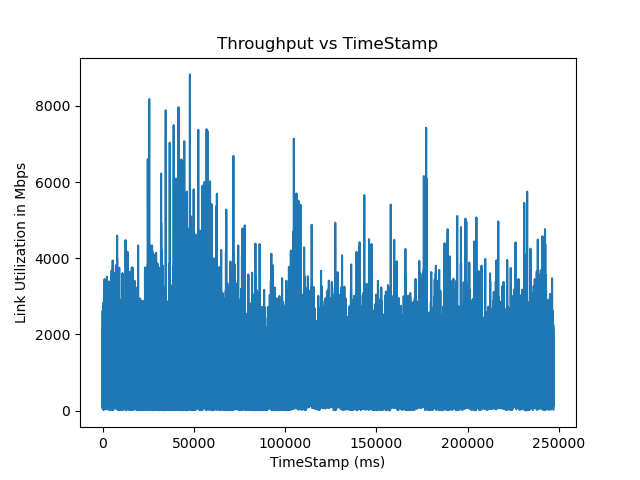
\includegraphics[width=0.75\textwidth]{Figures/link_util_600us.png}
    \caption[Link utilization for a trace]{Link utilization for a trace}
    \label{fig:linkutil}
    \bigskip
\end{figure}

Link utilization is a key metric in detecting congestion events in the network. If the bottleneck link becomes saturated, it can lead to congestion in the link. Link utilization can be computed in two ways. One method involves calculating the throughput for each packet i.e. \( n_b / (t_c - t_p) \) where \(n_b\) is the number of bytes in the packet and \(t_p\) and \(t_c\) are the timestamps of the previous and current packet respectively. Calculating the link utilization at the packet level can take a lot of time. We use a window and stride-based approach for calculating the link utilization. The throughput is calculated as \( \Sigma n_b / (t_w - t_1) \), where \( \Sigma n_b \) represents the sum of the number of bytes sent in the specified time window $w$ and, \(t_1\) and \(t_w\) represent the timestamp of the first and the last packet in the window respectively. The window is then moved by a stride $s$ (time-duration) and the process is repeated for the packets falling in the window. Figure \ref{fig:linkutil} shows the graph for Link Utilization (in Mbps) vs the Timestamp (in ms) for one of the traces captured at our server.

\begin{figure}[t]
    \centering
        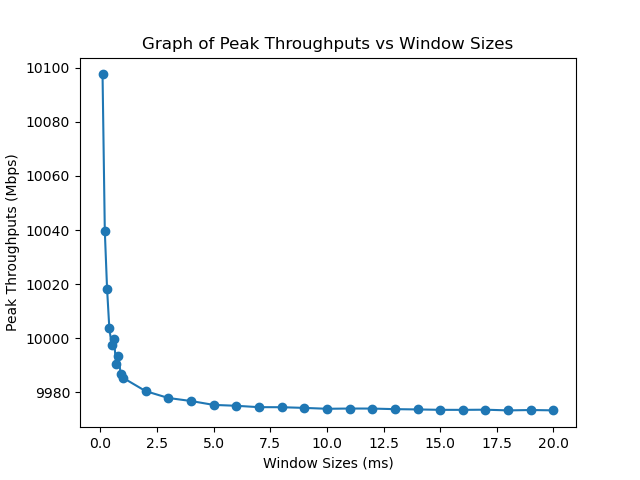
\includegraphics[width=0.75\textwidth]{Figures/peak_vs_window.png}
    \caption[Peak throughput vs window size]{Peak throughput vs window size}
    \label{fig:peak}
    \bigskip
\end{figure}

One of the key challenges while calculating link utilization is to calculate the appropriate window and stride sizes. The approach we used for calculating the suitable window size involved plotting a graph of peak throughput vs the window size in ms. If the window size is too small, it might even be less than the time it takes for a packet to serialize on the link and we will get very large throughput values. If the window size is too large, the peaks will get averaged out and we will get lower throughput values. Thus, the correct estimation of window size is necessary. Figure \ref{fig:peak} shows the optimal window size to be around 0.4 ms, as it is the first point at which the peak throughput is less than the link capacity ($10 Gbps$), and the time window is greater than the time it takes for a packet to serialize. Also, this is the point at which the slope of the graph decreases drastically. The time window is also not large enough to average out peak throughputs. We choose the stride size as half the window size for simplicity.
%----------------------------------------------------------------------------------------

\section{RTT}

RTT calculation is another key metric that also helps in congestion detection. The increase in the RTT of a flow can be attributed to a congestion event. Algorithm \ref{alg:rtt} showcases the approach we use to calculate RTT for different flows throughout their lifetime, which is inspired by Dart~\cite{dart-sigcomm22}.

\begin{algorithm}[ttpb]
\bigskip
\begin{algorithmic}
\State initialize $packettracker$,$rangetracker$ \Comment{intitialization of the two hash tables}
\State read $packet_d$ from $downlink$
\State read $packet_u$ from $uplink$
\While{$downlink$ and $uplink$}
\If{\(packet_d.ts < packet_u.ts\)}
    \If{\(expectedack > rangetracker[flow].right\)}
        \State $rangetracker[flow].right \gets expectedack$
        \State $packettracker[flow] \gets packet_d.ts$
    \Else 
        \State $rangetracker[flow].left \gets rangetracker[flow].right$
    \EndIf
    \State read $packet_d$ from $downlink$
\Else
    \If{$ack$ between $rangetracker[flow].left$ and $rangetracker[flow].right$}
        \State $rangetracker[flow].left \gets ack$
        \State $RTT \gets packet_u$ - $packettracker[flow]$
    \ElsIf{$ack$ == $rangetracker[flow].left$}
        \State  $rangetracker[flow].left \gets rangetracker[flow].right$
    \EndIf
    \State read $packet_u$ from $uplink$
\EndIf
\EndWhile
\end{algorithmic}
\caption[RTT calculation]{RTT calculation}
\label{alg:rtt}
\bigskip
\end{algorithm}

\begin{figure}[t]
    \centering
        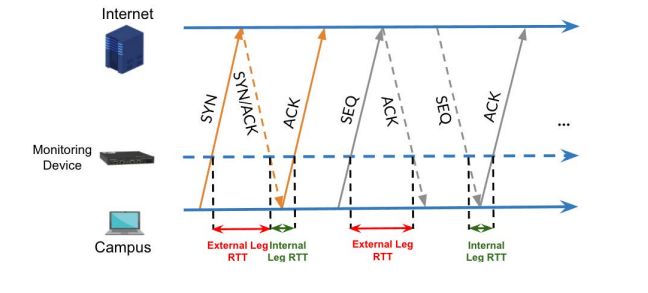
\includegraphics[width=0.8\textwidth]{Figures/rtt.png}
    \caption[RTTs of different legs]{RTTs of different legs ~\cite{dart-sigcomm22}}
    \label{fig:rtt}
    \bigskip
\end{figure}

The algorithm maintains two hash tables: the $packettracker$ table and the $rangetracker$ table for a flow. The $packetracker$ table stores the timestamps for the data packets belonging to a flow and matches the corresponding ACK packets to calculate and store the $RTT$. The $rangetracker$ table ensures that there are no ambiguous $RTT$ measurements. It maintains a range of valid sequence numbers for a flow, where the left edge represents the last ACKed byte by the receiver, and the right edge represents the last byte sent by the sender. The left edge moves when a new packet is ACKed, and the right edge moves when a new packet is sent. If the sequence number of data packet is less than the right edge or if the acknowledgment number of an ACK packet is equal to the left edge, we collapse the range to make it equal to the right edge. This is because these events indicate a packet loss event and can result in inflated RTT measurements for the packets falling in the range. The algorithm described above calculates the internal leg of the RTT as shown in figure \ref{fig:rtt}.

To calculate the complete leg RTT, we need to include the external leg RTT as well in our RTT calculation. We can calculate the complete RTT of a flow, by monitoring the TCP handshake. The time difference between the appearance of the SYN packet and the appearance of the ACK packet in the handshake will give us the complete leg RTT of the flow. The complete leg RTT will be required for packet loss detection as discussed later in the thesis. To detect congestion events, plotting the internal leg RTTs and seeing their trends would suffice. Figure \ref{fig:rttcdf} shows the cumulative distribution function of the internal leg RTT values for a set of flows captured in the downlink pcap trace.


\begin{figure}[h]
    \centering
        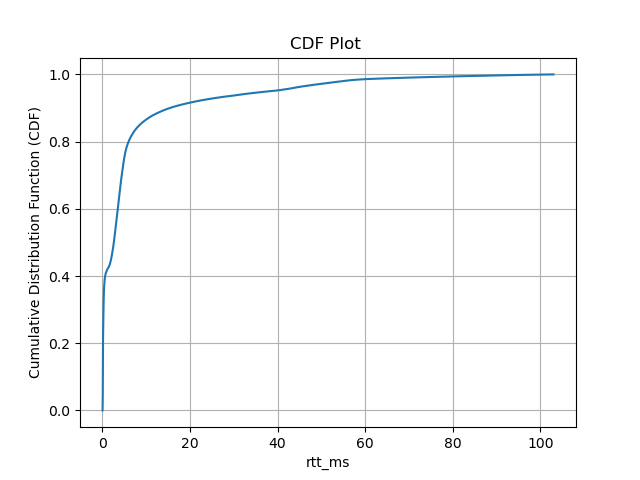
\includegraphics[width=0.75\textwidth]{Figures/rtt_cdf1.png}
    \caption[CDF of RTT in ms]{CDF of RTT in ms}
    \label{fig:rttcdf}
    \bigskip
\end{figure}

%----------------------------------------------------------------------------------------

\section{Packet Loss}

Packet loss is another important metric for detecting congestion events. High packet loss can imply queue buildup and hence, congestion in the network. We calculate packet losses at points both before and after our tapping point in the network. The packet losses occurring after the tapping point i.e. inside the campus network will be seen as a re-transmission event in the downlink pcap trace. The packet losses occurring before the tapping point i.e. on the internet side, can be seen as re-ordering events in the downlink trace. The approach for calculating losses inside the campus is pretty straightforward as we just have to detect retransmission events. We maintain a hash table corresponding to every packet using the flow four-tuple and the packet sequence number and record the time instance when see another packet of the same flow with the same sequence number. For calculating the losses on the internet side, we use a hole-filling-based approach. Algorithm \ref{alg:packet loss} showcases our approach to calculate packet loss on the internet side.

\begin{algorithm}[htpb]
\bigskip
\begin{algorithmic}
\State initialize hash-tables $nextsequencenumber$,$holes$ \Comment{Hash-tables per flow}
\For{$packet$ in $pcap$}
\For{$hole$ in $holes$}
\If{$packet.sequencenumber$ between $hole.start$ and $hole.end$}
    \If{\(packet.ts - hole.ts \geq packet.RTT\)}
        \State record $packet.ts$
        \State increment $internetloss$
    \EndIf
\EndIf 
\EndFor
\If{$nextsequencenumber[flow] \neq packet.nextsequencenumber$} 
    \State $hole.ts \gets packet.ts$
    \State $hole.start \gets nextsequencenumber[flow]$
    \State $hole.end \gets packet.nextsequencenumber$
    \State $holes[flow] \gets hole$
\EndIf

$nextsequencenumber[flow] \gets packet.nextsequencenumber$
\EndFor
\State state $internetloss$
\end{algorithmic}
\caption[Packet Loss]{Packet Loss}
\label{alg:packet loss}
\bigskip
\end{algorithm}

Here, $nextsequencenumber$ and $holes$ are hash tables that store, the next expected sequence number and the different holes encountered for a flow respectively. The key thing in the algorithm is to differentiate between in-network re-ordering and packet loss events. The time between the appearance of the hole and the actual packet is used to differentiate between the two events. Using the RTT estimation algorithm described above, we check if the time difference \( (t_p - t_h) \geq  RTT \), where $t_p$ is the time when the packet actually arrived and $t_h$ is the time when it was expected to arrive. If the condition is satisfied, then it's a packet loss event, otherwise it is an in-network re-ordering event. This is because it will take at least an RTT amount of time for the packet to get re-transmitted if it has been lost. While calculating packet losses, we also need to make sure the packet which we are looking at, is a data packet. We check this by looking at the payload length of a packet. The minimum size of a packet to be transmitted over the Ethernet is 60 bytes(excluding the checksum). The size of an ACK packet is 54 bytes, hence a 6-byte padding is added at the end of an ACK packet. We check if the payload length i.e. \( (packetlen - headerlen - 4) > 6 \), (where 4 bytes is the checksum size) to classify the packet as a data packet and then run the above algorithm on it. We finally report the internet side loss and the campus side loss at the end.

%----------------------------------------------------------------------------------------

\section{Other Key Metrics}

Several other metrics help us in better understanding the characteristics of TCP internet traffic and are useful meta-data for creating new algorithms.

\subsection{Asymmetry}

Detecting asymmetry is an important factor to look into to understand a network. It can happen at times, that a packet flows through a different router in its downlink journey, but takes a different path during its uplink journey. Asymmetry in a network can affect the calculation of metrics such as RTT measurement, as they rely on both the uplink and downlink traffic.

\begin{algorithm}[ttpb]
\bigskip
\begin{algorithmic}
\State initialize hashtable $synpackets$ \Comment{SYN packets for each flow}
\State $asymmetricflows \gets 0$
\For{$packet$ in $uplink$}
    \If{$packet$ is $SYN$}
        \State $synpackets[flow] \gets 1$
    \EndIf
\EndFor
\For{$packet$ in $downlink$}
    \If{$packet$ is $SYN-ACK$}
        \If{$flow$ not in $synpackets$}
            \State increment $asymmetricflows$
        \Else
            \State remove $flow$ from $synpackets$
        \EndIf
    \EndIf
\EndFor
\For{$flow$ in $synpackets$}
    \State increment $asymmetricflows$
\EndFor
\end{algorithmic}
\caption[Asymmetry Detection]{Asymmetry Detection}
\label{alg:asymmetry}
\bigskip
\end{algorithm}

Algorithm \ref{alg:asymmetry} shows how to detect asymmetry in a network. We maintain a hashtable of SYN packets corresponding to each flow and match the packets with the SYN-ACK packets. The number of unmatched packets gives us the amount of asymmetry.

\subsection{Flow Size, Duration and Number of Concurrent Flows}

Flow metrics like flow size, duration, and the number of concurrent flows are important meta-data used in the development of any new algorithm. We calculate the flow sizes by maintaining a hash table with the flow four-tuple as the key and the flow size, both in terms of number of packets and bytes as the value. We increment the flow size, whenever a new packet of the flow is encountered. We calculate the flow duration by maintaining a hash table with the flow four-tuple as the key and a pair of the flow start and end times as the value. The start time is set when we encounter the first packet of the flow. The end-time is updated whenever a new packet of the flow is encountered. We also set a $timeout value$, the time after which, if no more packets of the flow are seen, the flow is considered to end. The flow duration and sizes are reported when the flow ends. Algorithm \ref{alg:concurrent} shows how to calculate the number of concurrent flows at different intervals of time.

\begin{algorithm}[ttpb]
\bigskip
\begin{algorithmic}
\State populate arrays $startTimes,endTimes$ \Comment{pre-processed while calculating flow durations}
\State sort $startTimes,endTimes$
\State $concurrentflows \gets 0$
\State $time \gets stride$
\While{\(time < endTime\)}
\State $num_s \gets $ number of elements in $startTimes$ less than $time$
\State $num_e \gets $ number of elements in $endTimes$ less than $time$
\State $concurrentflows \gets num_s - num_e$
\State record $concurrentflows$
\State increment $time$ by $stride$
\EndWhile
\end{algorithmic}
\caption[Number of Concurrent Flows]{Number of Concurrent Flows}
\label{alg:concurrent}
\bigskip
\end{algorithm}

In the above algorithm, $num_s$ and $num_e$ can be calculated using binary search since the arrays $startTimes$ and $endTimes$ are sorted. The number of concurrent flows at a time is measured by calculating the difference between the number of flows with start time less than $time$ and the number of flows with end time less than $time$. We are basically subtracting the number of flows that have already ended from the number of flows that have started.


% \subsection{Congestion Duration and Inter-arrival time}

% We wrote scripts to analyze congestion duration and inter-arrival time. As we are tapping traffic after the gateway router, we can't see the queue that was formed at the router. We predict congestion by keeping track of N back-to-back packets at line rate where we experimentally determine the correct value of N to be set. We then compute the duration of such congestion events and the time after which the next congestion event occurs for a pcap trace.

%----------------------------------------------------------------------------------------